\documentclass[a4paper,11pt]{article}
\usepackage{algorithm}
\usepackage{algorithmic}

\usepackage{amsmath}
\usepackage{amssymb}

\usepackage[usenames,dvipsnames]{color}

\usepackage{eqparbox}

\usepackage{hyperref}

\usepackage{fullpage}

\usepackage{graphicx}

\usepackage{listings}
\lstset{language=bash}

\usepackage{natbib}

\usepackage{url}

%\newcommand\path[1]{#1} % Formats file names
\newcommand\code[1]{{\it #1}} % Typesets the name of a function, variable, class, etc.


\title{A Monte-Carlo AIXI Approximation: Tutorial}
\author{Daniel Visentin}



\begin{document}
\maketitle 

\tableofcontents

\newpage

\begin{abstract}
  MC-AIXI-CTW is an intelligent agent which learns through experience how to perform well in some environment. This includes, but is not limited to, games such as Tic Tac Toe, Pacman, or Kuhn Poker. MC-AIXI-CTW is an approximation of the universally optimal AIXI agent by \cite{hutter2005universal}. However, whereas the AIXI agent is incomputable (i.e.~it cannot be run on a computer), the MC-AIXI-CTW provides a graceful tradeoff between optimality and computational resources. That is, the more time and memory given to MC-AIXI-CTW, the better it performs.

The MC-AIXI-CTW software package provides a simple implementation of the MC-AIXI-CTW agent, several environments, and associated documentation with the goal of being simple to set up, use, and extend. This tutorial gives an introduction to the various components of the package, instructions on how to run the agent on the included environments, how to adjust the parameters that affect the agents learning performance, and how to add new environments/extend the agent.

\end{abstract}

\section{Introduction}
This document is designed to give a practical introduction to using the MC-AIXI-CTW software package. The package implements a simple version of the MC-AIXI-CTW agent from \cite{Hutter:11aixictwx}. Since the paper covers the agent in depth, we shall restrict ourselves to a brief non-technical overview of the agent before moving onto a tutorial of how to obtain/compile/run the agent. Following this will be more details on some of the aspects of running the agent as well as pointers on how to extend the code. For those who wish to get straight into running the agent, please see section \ref{sec:gettingstarted}.

\subsection{MC-AIXI-CTW}
The MC-AIXI-CTW agent seeks to interact intelligently within a particular environment. The environment can be just about anything, from a chess game to the entire universe. The agent interacts with the environment by performing actions (such as moving a piece on a chess board) and the environment interacts with the agent by providing observations (such as an image from a camera) and rewards for the agents actions. It is the goal of the agent to use its past interaction history to learn how to choose the actions which will lead to the greatest long-term reward.

There are two main components which combine to give the agent's action selection policy. The first is a model of the environment in which the agent attempts to model how the environment works and hence to predict how likely any given outcome is. Second is an algorithm for estimating the expected reward of each possible action by using the probabilities associated with the environment model. In particular, the MC-AIXI-CTW agent uses context-tree weighting for the environment model and the $\rho$UCT search algorithm for estimating the expected rewards. More details of these algorithms can be found in the original paper by \cite{Hutter:11aixictwx}.


\section{Getting started}
\label{sec:gettingstarted}
This section briefly outlines the process of getting the source code, compiling the code, running the agent on an environment, visualising the results, and generating the documentation. More details on the individual steps can be found in later sections.


\subsection{Step 1: Prerequisites}
\label{sec:prerequisites}

\subsubsection{Required}
The only thing required to use the MC-AIXI-CTW software is a C++ compiler. We will assume that you are using either g++ on Linux (\url{http://gcc.gnu.org}) or visual studio on windows (\url{http://microsoft.com/visualstudio/}).

\subsubsection{Optional}
The following utilities are not required for the use of the core code.
\begin{itemize}
\item {\bf Make:} Having the make utility (\url{http://gnu.org/software/make/}) on Linux will enable easier compilation.

\item {\bf Graphing:} The MC-AIXI-CTW package also comes with a python script for graphing the data, use of which is optional. In order to use the graphing utility, you must have a relatively recent version of python (\url{http://python.org}), numpy (\url{http://numpy.scipy.org}), and matplotlib (\url{http://matplotlib.sourceforge.net}). 

\item {\bf Documentation:} In order to generate the source code documentation, you must have a utility called doxygen (\url{http://doxygen.org}) and a suitable \LaTeX installation (\url{http://latex-project.org}). Doxygen extracts specially-formatted comments from within the source code in order to make the documentation. \LaTeX is used to typeset the formulas and PDF documentation.
\end{itemize}


\subsection{Step 2: Getting the code}


\subsubsection{Linux}
Download the archive. Extract it into a directory called \path{mc-aixi-ctw} using the following command
\begin{lstlisting}[frame=single]
tar -xf mc-aixi-ctw.tar.gz
\end{lstlisting} % Archive created with "tar -czf mc-aixi-ctw.tar.gz mc-aixi-ctw/"
For the duration of this tutorial we shall specify all file paths relative to the \path{mc-aixi-ctw} directory.


\subsubsection{Windows}
Download the archive. Extract the zip folder and open the solution file \path{mc-aixi-ctw.sln} in Visual Studio.


\subsection{Step 3: Compiling the code}
\subsubsection{Linux}
Compiling the code on Linux requires a C++ compiler and (optionally) the ``make'' utility. Assuming you have both of these, the code can be compiled simply by running the command:
\begin{lstlisting}[frame=single]
make
\end{lstlisting}
from within the \path{mc-aixi-ctw} directory. This will result in the creation of the \path{aixi} executable within the \path{mc-aixi-ctw} directory. Because the make command avoids recompiling code that has not changed, it is necessary to clean the results of a compilation in order to recompile everything from scratch:
\begin{lstlisting}[frame=single]
make clean
make
\end{lstlisting}
While this is not always necessary, some changes to the source code might require a complete recompilation.

Alternatively, in the absence of the make command, one can use a compiler directly. The appropriate command for g++ is:
\begin{lstlisting}[frame=single]
g++ -O3 -Wall -o aixi src/*.cpp
\end{lstlisting}


\subsubsection{Windows}
To compile the code, simply press F7. This is not a necessary step as running the code from within Visual Studio will automatically compile it.


\subsection{Step 4: Running the code}


In order to run the code and have it do something useful, it is necessary to specify a few configuration options. Most importantly, the environment for the agent to interact with and the agent's search parameters. Several example configuration files are available from the \path{conf} directory, one for each environment. Details of all the configuration parameters and their possible values can be found in section \ref{sec:options}. For now, we will run the agent on a maze environment using one of the example configuration files. The environment consists of a $4 \times 4$ empty maze, the bottom-right corner of which is the ``goal state.'' The agent is able to move around the maze using the four cardinal directions (up, down, left, right). Reaching the goal state gives the agent a reward and transports it to another square at random.

\subsubsection{Linux}
Running the agent is as simple as invoking the following command from within the \path{mc-aixi-ctw} directory:
\begin{lstlisting}[frame=single]
./aixi conf/maze-4x4.conf log/maze-4x4.log
\end{lstlisting}
In this example, \path{./aixi} refers to the executable we compiled in the previous step, \path{conf/maze-4x4.conf} is  configuration file for the $4 \times 4$ maze environment, and \path{log/maze-4x4.log} is the file to which the agent will log its progress. The agent-environment interaction can be stopped at any time by pressing Ctrl-C (or otherwise stopping the process) or at a particular time using certain configuration options (see section \ref{sec:options}).


\subsubsection{Windows}
\begin{figure}[hp]
  \begin{center}
    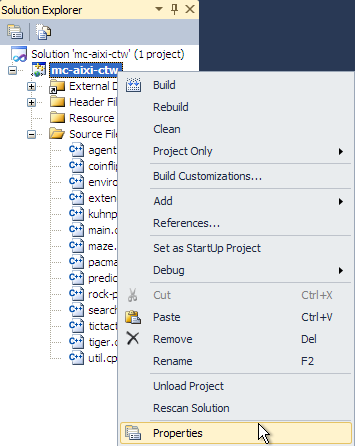
\includegraphics[width=10cm]{img/properties.png}
    \caption{Project properties}
    \label{fig:properties}
  \end{center}
\end{figure}
\begin{figure}[hp]
  \begin{center}
    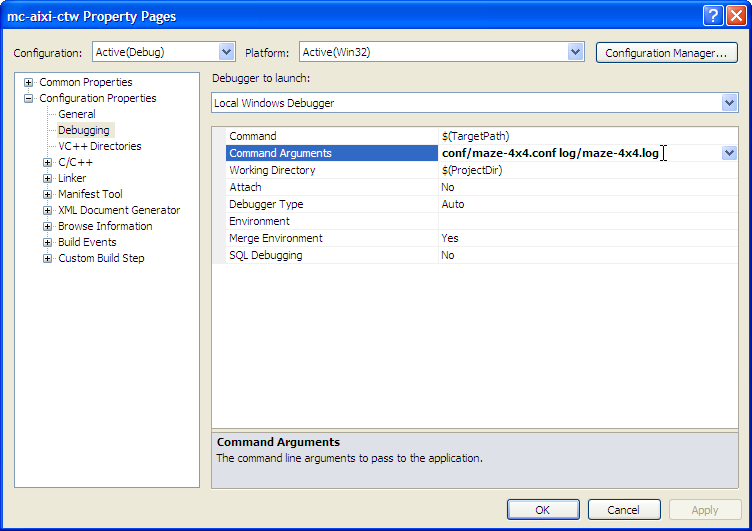
\includegraphics[width=16cm]{img/arguments.png}
    \caption{Command-line arguments}
    \label{fig:arguments}
  \end{center}
\end{figure}

There are two steps in running the code from visual studio. First, to specify command-line arguments, select the mc-aixi-ctw project in the solution explorer, right-click on it and select the properties option (figure \ref{fig:properties}). Then, under Configuration Properties select Debugging. Edit the Command Arguments option (figure \ref{fig:arguments}) so that it reads
\begin{lstlisting}[frame=single]
conf/maze-4x4.conf log/maze-4x4.log
\end{lstlisting}
The first argument gives the configuration file for the environment while the second gives the file to which the agent will log its progress. Exit from the properties dialog by clicking OK. Now to run the code simply press F5 or click on the play button in the toolbar.





\subsection{Step 5: Visualising the results (Optional)}
Having run the agent, the results of the agent's interaction are available in the log file \path{log/maze-4x4.log}. The log file is a comma-separated-value (CSV) file with one line per cycle of interaction plus an initial header line. The header line gives the names of the quantities logged to the file while the all the other lines give the corresponding values for a particular cycle. 

Provided with the source code is a graphing utility that enables you to visualise the results. Alternatively, you can use your own selection of tools (e.g.~excel or matlab) to analyse the data. The graphing utility has certain prerequisites in addition to those of the agent, these are detailed in section \ref{sec:prerequisites}. Running the graphing utility is simply a matter of invoking the following command
\begin{lstlisting}[frame=single]
python graph.py
\end{lstlisting}
from within the mc-aixi-ctw folder. The graphing utility will generate a set of graphs for each log file in the \path{log} directory, each of which will be placed in a sub-directory of the \path{graph} directory. 




\subsection{Step 6: Generating documentation (Optional)}
Generating the HTML and PDF documentation requires the use of doxygen and \LaTeX~as detailed in section \ref{sec:prerequisites}. These utilities extract specially-formatted comments from the code and compile them into a set of web pages or a PDF for easy viewing. To generate the documentation, simply run the command
\begin{lstlisting}[frame=single]
doxygen mc-aixi-ctw
\end{lstlisting}
from within the \path{doc} directory. The HTML documentation can be viewed by opening the file \path{doc/html/index.html} in a web browser. The \LaTeX~documentation requires an initial compilation step:
\begin{lstlisting}[frame=single]
pdflatex refman.tex
\end{lstlisting}
run from within the \path{doc/latex} directory. The PDF documentation can then be accessed by viewing the file \path{doc/latex/refman.pdf}.



\section{Configuration options}
\label{sec:options}
The program is configured through the use of key/value pairs in a configuration file. Each line of the file may contain at most one assignment of the form
\begin{lstlisting}[frame=single]
key = value
\end{lstlisting}
with any character following a \# being ignored as a comment. In order to tell the program which configuration file to use, the path of the configuration file is passed as the first command-line argument to the executable. For example, to use a file \path{conf.conf} we would invoke
\begin{lstlisting}[frame=single]
./aixi conf.conf
\end{lstlisting}

Configuration options can be separated into a number of categories which we shall address below. Example configuration files can be found in the \path{conf} directory.


\subsection{Agent configuration}
These options configure the agent, particularly the effort it puts into searching for the optimal action.
\begin{itemize}
\item {\bf agent-horizon:} The depth of the agent's search horizon. When the agent considers choosing a particular action, it estimates the action's consequences a certain number of cycles into the future. The search horizon specifies the maximum number of cycles to look ahead. {\em Default value:} 5. {\em Valid values:} positive integers.

\item {\bf ct-depth:} The maximum depth of the context tree used by the agent. Larger values enable the agent to more accurately model complex environments but require increased computation and memory resources. {\em Default value:} 30. {\em Valid values:} positive integers.

\item {\bf exploration:} The probability that the agent chooses an action at random instead of using the $\rho$UCT search. {\em Default value:} 0.0 (i.e.~no exploration). {\em Valid values:} decimal values between 0.0 and 1.0 inclusive.

\item {\bf explore-decay:} The rate at which the exploration probability decreases each cycle. In particular, if $e$ is the initial exploration probability and $c$ is the explore-decay then the exploration rate after cycle $t$ is $c^t e$. {\em Default value:} 1.0 (i.e.~no decay). {\em Valid values:} decimal values between 0.0 and 1.0 inclusive.

\item {\bf mc-simulations:} The number of Monte-Carlo simulations to perform when choosing an action. More simulations are more likely to give accurate estimates of each actions expected utility but require increased computation and memory resource usage. {\em Default value:} 300. {\em Valid values:} positive integers.

\item {\bf terminate-age:} The number of cycles of interaction between the agent and environment. When this number is reached, the program terminates. A value of 0 will cause the agent and environment to interact indefinitely. {\em Default value:} 0. {\em Valid values:} nonnegative integers.
\end{itemize}

\subsection{Environment configuration}
These options specify general environment properties. See the subsections for options which apply to specific environments.
\begin{itemize}
\item {\bf environment:} Determines which environment the agent will interact with. {\em Valid values:} coin-flip, extended-tiger, kuhn-poker, maze, pacman, rock-paper-scissors, tictactoe, tiger.

\item {\bf action-bits/observation-bits/percept-bits/reward-bits:} Specifies the maximum number of bits needed to encode an action/observation/percept/reward. These are set by the environment when it is created.

\item {\bf max-action/max-observation/max-reward:} Actions, observations, and rewards are passed between the agent and environment as nonnegative integers. These options specify the maximum action that can be sent to the environment and the maximum observation/reward that can be received from the environment. These are set by the environment when it is created.
\end{itemize}


\subsubsection{Coin-flip:}
The coin-flip environment involves the environment flipping a biased coin and the agent attempting to predict which side it will land on.
\begin{itemize}
\item {\bf coin-flip-p:} The probability of the biased coin landing on heads. {\em Default value:} 0.7. {\em Valid values:} Decimal values between 0.0 and 1.0 inclusive.
\end{itemize}

\subsubsection{Extended tiger:}
\begin{itemize}
\item {\bf tiger-listen-accuracy:} The probability that listening for the tiger while seated will correctly identify which door the tiger is behind. {\em Default value:} 0.85. {\em Valid values:} Decimal values between 0.0 and 1.0 inclusive.
\end{itemize}

\subsubsection{Maze:}
The maze environment represents a maze through which the agent must navigate. Configuration involves specifying the structure of the maze, the rewards the agent receives from each square, as well as the type of observations given to the agent. Examples configuration files include \path{conf/cheesemaze.conf} and \path{conf/maze-4x4.conf}.
\begin{itemize}
\item {\bf maze-num-rows:} The number of rows in the maze. {\em Valid values:} Nonnegative integers.

\item {\bf maze-num-cols:} The number of columns in the maze. {\em Valid values:} Nonnegative integers.

\item {\bf maze-layout$n$:} The structure of row $n$ of the maze ($1 \le n \le \text{maze-num-rows}$). The value should be a contiguous sequence containing maze-num-cols symbols as follows:
  \begin{itemize}
  \item {\bf @} Represents an impassable square in the maze.

  \item {\bf *} Represents an empty square which can be teleported to.

  \item {\bf \&} Represents an empty square which cannot be teleported to.

  \item {\bf !} Represents an empty square which can be teleported from.
  \end{itemize}
  If the agent moves into a {\bf !} square it will teleport at random to a {\bf *} square. The maze must contain at least one square capable of being teleported to.

\item {\bf maze-rewards$n$:} Comma-separated list of rewards for each square in row $n$ ($1 \le n \le \text{maze-num-rows}$). If the agent enters (or attempts to enter) a particular square, it receives the corresponding reward, regardless of whether it can actually enter the square or not. Rewards are translated by the program so that the minimum reward in the maze has value 0. {\em Valid values:} Integers.

\item {\bf maze-observation-encoding:} The type and encoding of observations received by the agent. {\em Valid values:}
  \begin{itemize}
  \item {\bf uninformative:} The agent receives the same observation each cycle.

  \item {\bf walls:} The agent receives an observation specifying whether there are walls ({\bf @}) above, below, left, or right of its current position.

  \item {\bf coordinates:} The observation specifies the coordinates of the agent in the maze.
  \end{itemize}
\end{itemize}



\subsubsection{Tiger:}
\begin{itemize}
\item {\bf tiger-listen-accuracy:} The probability that listening for the tiger will correctly identify which door the tiger is behind. {\em Default value:} 0.85. {\em Valid values:} Decimal values between 0.0 and 1.0 inclusive.
\end{itemize}



\subsection{Miscellaneous}
These options do not apply directly to either the agent or environment.
\begin{itemize}
\item {\bf random-seed:} Used to set the random seed of the program. Repeatedly using the same value across different runs of the program should (assuming no other changes) result in the same sequence of generated random numbers and hence the same sequence of interactions between the agent and environment. {\em Default value:} 0. {\em Valid values:} nonnegative integers.

\item {\bf verbose:} Determines whether the program logs interaction information to the standard output as well as to the log file. When debugging, it is useful to set this option to true so as to see what is happening between the agent and environment. {\em Default value:} false. {\em Valid values:} true, false.
\end{itemize}


\section{Log format}
The agent-environment interaction is logged to a file in comma-separated value (CSV) format. Each line in the log file corresponds to an interaction cycle except for the first line which is a list of the names of the values being logged. The field names are as follows:
\begin{itemize}
\item {\bf cycle:} The interaction cycle which the current line refers to. Numbered beginning from 1.

\item {\bf observation:} The observation received by the agent represented as an integer.

\item {\bf reward:} The reward received by the agent.

\item {\bf action:} The action taken by the agent represented as an integer.

\item {\bf explored:} 1 if the agent explored (i.e.~chose an action at random) and 0 otherwise (i.e.~the agent searched for an action).

\item {\bf explore rate:} The current exploration rate (probability that the agent will explore this cycle).

\item {\bf total reward:} The total reward accumulated by the agent up to and including this cycle.

\item {\bf average reward:} The average reward received by the agent from all cycles up to and including the current cycle.

\item {\bf time:} The time (in seconds) elapsed over the cycle.

\item {\bf model size:} The number of nodes in the agent's context-tree model.
\end{itemize}
To direct the program to log at a particular location (e.g. \path{log/mylog.log}), provide the path as the second command-line argument to the executable:
\begin{lstlisting}[frame=single]
./aixi conf.conf log/mylog.log
\end{lstlisting}


\section{Extending the code}
This section will give some brief pointers about where to start if you wish to add something to/change the code.

\subsection{Adding a new environment}
We will detail the steps required to create and integrate a new environment into the code. It might be helpful to look at the coin flip environment which is a relatively simple example. For illustration purposes, we will assume the environment is called ``jumping castle.''
\begin{enumerate}
\item {\bf Create files:} Create a new code (.cpp) and header (.hpp) file for your environment in the \path{src} folder. For example, \path{src/jumping-castle.cpp} and \path{src/jumping-castle.hpp}.

\item {\bf Update makefile (optional):} If you use the make command to compile your code, it is necessary to update the makefile so it knows to compile your new environment. To do this, simply append ``\path{src/jumping-castle.o}'' to line in \path{Makefile} beginning with ``aixi:''.

\item {\bf Include the environment:} Open the file \path{src/main.cpp} and locate the \#include section at the top of the file. You should see a block of \#include statements relating to environments. Add the line
  \lstset{language=c++}
  \begin{lstlisting}[frame=single]
#include "jumping-castle.hpp"
  \end{lstlisting}
  to this block. You should also add this line to the top of the \path{src/jumping-castle.cpp} file you previously created.

\item {\bf Inherit from the Environment class:} All environments must inherit from the Environment class (\path{src/environment.hpp}). This is done by adding the line
  \begin{lstlisting}[frame=single]
#include "environment.hpp"
  \end{lstlisting}
  to the top of \path{src/jumping-castle.hpp} and creating a new class to represent the new environment:
  \begin{lstlisting}[frame=single]
class JumpingCastle : public Environment {};
  \end{lstlisting}
  Within the newly created class you must define a number of methods (in \path{src/jumping-castle.hpp}) and implement them (in \path{src/jumping-castle.cpp}). In particular:
  \begin{itemize}
  \item {\bf Constructor:} Create the constructor with prototype
    \begin{lstlisting}[frame=single]
JumpingCastle(options_t &options);      
    \end{lstlisting}
    The constructor will be passed the dictionary of configuration options. It will then set-up the environment and assign an initial observation and reward to the variables m\_observation and m\_reward (inherited from Environment).

  \item {\bf Action/Observation/Reward range:} The new environment must specify the range of possible actions, observations, and rewards. Since the code can only handle interactions represented by nonnegative integers, it is simply a matter of specifying the maximum value of each type of interactions. This is done by inheriting the methods maxAction(), maxObservation(), and maxReward() from the Environment class and having them return the appropriate values. As an example, assume the jumping castle environment has two possible actions: jump and bounce. We might assign these actions to the values 0 and 1 respectively, in which case we would have maxAction() return 1.

  \item {\bf performAction():} The performAction() method is perhaps the most important thing to implement. The method takes an agents action and calculates the next percept (observation and reward), placing the values in the variables m\_observation and m\_reward. The function is inherited from the Environment class and has prototype
    \begin{lstlisting}[frame=single]
virtual void performAction(action_t action);
    \end{lstlisting}

  \item {\bf Define a print() function (optional):} The Environment class provides a default print function which returns a string representation of the current state of the class. Overriding this method enables the environment to return a more tailored representation but is not required.

  \end{itemize}

\item {\bf Enable the environment:} The final step is to allow the environment to be selected. Open the \path{src/main.cpp} file and navigate to the main() function. Within this function is a large if statement where each condition checks the value of the environment\_name variable against a particular environment. You need to add a test for your new environment of the form
    \begin{lstlisting}[frame=single]
else if (environment_name == "jumping-castle") {
    env = new JumpingCastle(options);
}
    \end{lstlisting}


  \item {\bf Compile and run:} Compile the code with the commands
    \lstset{language=bash}
    \begin{lstlisting}[frame=single]
make clean
make
    \end{lstlisting}
    At this stage you will have to fix any compilation errors due to your code before you continue.

Create a new configuration file \path{conf/jumping-castle.conf} that includes the line
    \begin{lstlisting}[frame=single]
environment = jumping-castle
    \end{lstlisting}
and an appropriate selection of other options. 

Run the executable with
    \begin{lstlisting}[frame=single]
./aixi conf/jumping-castle.conf log/jumping-castle.log
    \end{lstlisting}
\end{enumerate}



\subsection{Changing the environment model}
The MC-AIXI-CTW agent models the environment using a context-tree. The code related to the model is contained in the CTNode and ContextTree classes within the \path{src/predict.cpp} and \path{src/predict.hpp} files. In changing/extending the model, it is necessary to keep in mind that:
\begin{itemize}
\item The model will be updated each cycle with the most recent action and percept. Thus, each update should be efficient and the model size should not grow without bound. Furthermore, it should be possible to efficiently revert the model to a previous state.

\item The model should be able to calculate the probability of future interaction sequences and to sample from this distribution.
\end{itemize}


\subsection{Changing the action selection policy}
The MC-AIXI-CTW agent uses the $\rho$UCT search algorithm to choose an action each cycle. Each sample is performed using the SearchNode class from the \path{src/search.cpp} and \path{src/search.hpp} files. The number of samples and ultimate action selection is handled by the search() method of the Agent class from the \path{src/agent.cpp} and \path{src/agent.hpp} files. Finally, the playout() method of the Agent class is used to give an initial reward estimate for future interaction sequences. It is used the first time a particular interaction sequence is sampled by the $\rho$UCT algorithm. Ideally, the playout policy should be computationally efficient. For example, the default playout policy chooses actions at random for its sample. In changing how action selection is performed it is possible to change some but not all of these components.


\subsection{Logging additional data}
Logging is done in the inner loop of the mainLoop() function (\path{src/main.cpp}) using the logger stream. To change what is being logged, simply locate the statements involving logger and make the necessary changes.


\subsection{Efficiency}
This implementation of MC-AIXI-CTW values simplicity over efficiency. For this reason there are several possible extensions/changes to the codebase that will result in a quicker agent. For example, the algorithm creates and deletes a lot of nodes in the context tree during the search phase. This can be made more efficient by using a preallocation of nodes, or modifying the context tree to support copy-on-write. A more substantial improvement would involve parallelising the search code.


\section{About}
This project developed out of an assignment during the COMP4620/8620 advanced topics in artificial intelligence course at the Australian National University (\url{http://cs.anu.edu.au/courses/COMP4620/2010.html}). The goal was to develop a simplified version of the MC-AIXI-CTW agent using C++.

\subsection{Acknowledgements}
The MC-AIXI-CTW algorithm was developed by \cite{Hutter:11aixictwx}. The code in this project is based on the more heavy-weight implementation by Joel Veness (\url{http://jveness.info/software/default.html}). Thanks go to the following students who participated in the coding of the algorithm: Chirag Chatbar, Mayank Daswani, Aaron Defazio, Sotirios Diamand, Nitin Gupta, Jonathon Hunklinger, Qiaochu Li, Xiang Li, Joseph Noel, Alexander Fergus O'Neill, Karunanithi Prabhu, Fatemeh Rajabiyazdi, Sam Rathmanner, Paul Rivera, Wen Shao. Phuong Nguyen supervised the students. Marcus Hutter provided many useful comments on the code, documentation, and tutorial. 



\newpage
\bibliographystyle{plainnat}
\bibliography{tutorial}

\end{document}
